% Presentación al equipo de investigación: cómo funciona el detector, qué tan bien detecta cada
% especie, en qué difieren sus detecciones de las anotaciones y el ciclo de mejora que se
% propone. En inglés. Las cifras, la tabla de Raven y las figuras salen de
% notebook/figuras_presentacion.ipynb (figures/); aquí no se escribe ningún número a mano.
% Compilar con `make slides` desde la raíz del repositorio.
\documentclass[aspectratio=169,10pt,xcolor=table]{beamer}

\usepackage[T1]{fontenc}
\usepackage[sfdefault,lining,semibold]{FiraSans}
\usepackage[scale=0.9]{FiraMono}
\usepackage{booktabs}
\usepackage[skins]{tcolorbox}
\usepackage{fontawesome5}
\usepackage{tikz}
\usetikzlibrary{arrows.meta,calc,patterns,positioning}

\graphicspath{{figures/}}
% generado por notebook/figuras_presentacion.ipynb; no editar
\newcommand{\threshold}{0.11}
\newcommand{\recall}{0.81}
\newcommand{\precision}{0.67}
\newcommand{\mapThirty}{0.62}
\newcommand{\speciesCorrect}{99}
\newcommand{\callCorrect}{98}
\newcommand{\testBoxes}{7,931}
\newcommand{\testRecordings}{601}
\newcommand{\nModels}{4}
\newcommand{\nClasses}{25}
\newcommand{\realtime}{501}
\newcommand{\gpuName}{NVIDIA RTX A5500}
\newcommand{\minCount}{100}
\newcommand{\nTrained}{25}
\newcommand{\nNotTrained}{13}
\newcommand{\ccAnnotations}{29}
\newcommand{\ccRecordings}{7}
\newcommand{\ccMissing}{71}
\newcommand{\nCovered}{11}
\newcommand{\coveredShare}{70}
\newcommand{\nDetections}{6,768}
\newcommand{\nAnnotations}{5,343}
\newcommand{\nMissed}{1,361}
\newcommand{\pctFound}{75}
\newcommand{\pctMissed}{25}
\newcommand{\labelSameSpecies}{62}
\newcommand{\topConfusion}{sb/pcc $\to$ sb/ppc}
\newcommand{\topConfusionN}{22}
\newcommand{\nMatch}{3,982}
\newcommand{\pctMatch}{59}
\newcommand{\nBox}{191}
\newcommand{\pctBox}{3}
\newcommand{\nLabel}{146}
\newcommand{\pctLabel}{2}
\newcommand{\nNone}{2,449}
\newcommand{\pctNone}{36}
\newcommand{\corpusNone}{11,864}
\newcommand{\corpusNoneHalf}{236}
\newcommand{\corpusNonePerHour}{735}
\newcommand{\ciLow}{0.74}
\newcommand{\ciHigh}{0.86}
\newcommand{\repoUrl}{github.com/nhrot-fc/tesis-primate}


% La paleta de las figuras del cuaderno: mismas cuatro categorías y misma escala de recall.
\definecolor{ink}{HTML}{17252B}
\definecolor{muted}{HTML}{5F6B70}
\definecolor{paper}{HTML}{F7F5EF}
\definecolor{rule}{HTML}{DDD6C6}
\definecolor{track}{HTML}{E6E1D4}
\definecolor{match}{HTML}{008A9E}
\definecolor{boxdiff}{HTML}{C98419}
\definecolor{calldiff}{HTML}{7B5FB0}
\definecolor{nothing}{HTML}{C64B36}
\definecolor{missed}{HTML}{C9C1AF}
\definecolor{warm}{HTML}{A9520F}
\definecolor{tierhigh}{HTML}{006E7F}
\definecolor{tiermid}{HTML}{4FAFBF}
\definecolor{tierlow}{HTML}{A9D6DE}

\setbeamercolor{background canvas}{bg=paper}
\setbeamercolor{normal text}{fg=ink}
\setbeamercolor{frametitle}{fg=ink}
\setbeamerfont{frametitle}{size=\Large,series=\bfseries}
\setbeamertemplate{navigation symbols}{}
\setbeamersize{text margin left=8mm,text margin right=8mm}
\setbeamertemplate{frametitle}{\vspace*{5mm}\insertframetitle\par}
\setbeamertemplate{footline}{%
  \hfill{\color{muted}\scriptsize\insertframenumber}\hspace*{8mm}\vspace*{3mm}}

\newcommand{\code}[1]{\texttt{#1}}
\newcommand{\swatch}[1]{\tikz[baseline=-0.6ex]\fill[#1] (0,-0.8mm) rectangle (3.2mm,0.8mm);}
% Una cifra grande con su rótulo debajo
\newcommand{\metric}[2]{%
  \begin{minipage}[t]{20mm}\centering
    {\fontsize{22}{24}\selectfont\bfseries\color{match}#1}\\[0.6mm]
    {\scriptsize\color{muted}#2}
  \end{minipage}}
% Una etiqueta de color para lo que decide el equipo
\newcommand{\chip}[3][white]{{\setlength{\fboxsep}{1.8pt}\colorbox{#2}{\scriptsize\bfseries\color{#1}#3}}}

% Un ejemplo de la diapositiva de contraste: color, nombre, cantidad, imagen y una línea
\newcommand{\showcase}[5]{%
  \begin{minipage}[t]{45.5mm}
    {\swatch{#1}\;\small\bfseries #2}\hfill{\small\color{muted}#3}\par\vspace{1mm}
    \includegraphics[width=\linewidth]{#4}\par\vspace{0.8mm}
    {\scriptsize\color{muted}#5}
  \end{minipage}}

% El círculo con ícono de cada etapa del ciclo
\tikzset{badge/.style={circle, fill=#1, text=white, minimum size=10mm, font=\normalsize}}

% Las tarjetas por especie (figures/tablas/especies.tex): todas del mismo ancho y alto, así que
% las ocho quedan alineadas en dos filas.
\newlength{\cardwidth}\setlength{\cardwidth}{34mm}
\newlength{\cardheight}\setlength{\cardheight}{24.5mm}
\newlength{\barlength}\setlength{\barlength}{14.5mm}
% El alto lo fija el minipage de adentro, para que \vfill lleve el pie al fondo
\tcbset{species card/.style={enhanced, nobeforeafter, box align=top, width=\cardwidth,
    arc=1.6mm, boxrule=0.4pt, colframe=rule, colback=white,
    left=1.8mm, right=1.8mm, top=1.4mm, bottom=1.2mm, boxsep=0pt}}
\newcommand{\diamondmark}{\tikz[baseline=-0.6ex]\fill[ink] (0,0) -- (0.65mm,0.65mm) --
  (1.3mm,0) -- (0.65mm,-0.65mm) -- cycle;}
\newcommand{\hatch}{\tikz[baseline=-0.6ex]\draw[rule, pattern=north east lines,
  pattern color=missed] (0,-0.7mm) rectangle (2.6mm,0.7mm);}
% #1 código, #2 nombre, #3 recall de la especie, #4 cajas de prueba, #5 renglones, #6 pie
\newcommand{\speciescard}[6]{%
  \begin{tcolorbox}[species card]
    \begin{minipage}[t][\cardheight][t]{\linewidth}
      {\scriptsize\bfseries #1\,\mdseries\color{muted}\textperiodcentered\,\textit{#2}\par}
      {\tiny\color{muted}recall #3 \textperiodcentered{} #4 test calls\par}\vspace{1mm}
      {\fontsize{7}{9.4}\selectfont #5\par}\vfill
      #6
    \end{minipage}
  \end{tcolorbox}}
% #1 llamada, #2 recall, #3 precisión, #4 color de la barra, #5 la cifra que se muestra
\newcommand{\callrow}[5]{%
  \makebox[7.5mm][l]{\ttfamily #1}%
  \tikz[baseline=-0.6ex]{%
    \fill[track] (0,-0.8mm) rectangle (\barlength,0.8mm);
    \fill[#4] (0,-0.8mm) rectangle ({#2*\barlength},0.8mm);
    \fill[ink] ({#3*\barlength},0) +(-0.65mm,0) -- +(0,0.65mm) -- +(0.65mm,0) --
      +(0,-0.65mm) -- cycle;}%
  \hfill #5\par}
\newcommand{\nottrained}[1]{{\tiny\color{muted}\hatch\ #1\par}}
% Una especie sin ningún tipo de llamada entrenado: #3 anotaciones, #4 grabaciones
\newcommand{\emptycard}[4]{%
  \begin{tcolorbox}[species card, frame hidden, colback=paper,
      borderline={0.5pt}{0pt}{warm, dash pattern=on 1.5pt off 1pt}]
    \begin{minipage}[t][\cardheight][t]{\linewidth}
      {\scriptsize\bfseries #1\,\mdseries\color{muted}\textperiodcentered\,\textit{#2}\par}
      \vspace{2mm}
      {\footnotesize\bfseries\color{warm}No call type trained\par}\vspace{1.5mm}
      {\scriptsize\raggedright\color{muted}Only #3 annotations, in #4 recordings; a call type
      needs \minCount.\par}
    \end{minipage}
  \end{tcolorbox}}

% Apéndice, arquitecturas: el intervalo de recall de cada modelo sobre un eje común
\newlength{\ciwidth}\setlength{\ciwidth}{24mm}
\newcommand{\ciplot}[3]{\tikz[baseline=-0.6ex]{%
  \draw[rule, line width=0.4pt] (0,0) -- (\ciwidth,0);
  \draw[match, line width=1.6pt] ({(#1-\ciLow)/(\ciHigh-\ciLow)*\ciwidth},0) --
    ({(#3-\ciLow)/(\ciHigh-\ciLow)*\ciwidth},0);
  \fill[ink] ({(#2-\ciLow)/(\ciHigh-\ciLow)*\ciwidth},0) circle (0.65mm);}}
\newcommand{\ciaxis}{\tikz[baseline=-0.6ex]{%
  \foreach \v in {0.75,0.80,0.85}{%
    \draw[muted] ({(\v-\ciLow)/(\ciHigh-\ciLow)*\ciwidth},0) -- ++(0,-0.6mm)
      node[below, inner sep=0.4mm, font=\tiny] {\v};}}}
% El \input primitivo, expandible: deja que la tabla generada empiece una fila con \rowcolor
\makeatletter\newcommand{\rawinput}[1]{\@@input #1 }\makeatother
\newcommand{\archcell}[2]{\begin{tabular}[t]{@{}l@{}}\textbf{#1}\\[-0.4mm]
  {\tiny\color{muted}#2}\end{tabular}}
% Apéndice, más ejemplos: imagen, clase, score, grabación, segundo
\newcommand{\moreexample}[5]{%
  \begin{minipage}[t]{45.5mm}
    \includegraphics[width=\linewidth]{#1}\par\vspace{0.6mm}
    {\scriptsize\code{#2}\;\textbf{#3}\hfill{\tiny\color{muted}#4 @ #5\,s}\par}
  \end{minipage}}

\title{Primate call detector}
\author{Fernando Candia}
\date{October 2026}

\begin{document}

% --------------------------------------------------------------------------------------------
\begin{frame}[plain]
  \vspace*{14mm}
  {\color{match}\small\bfseries PRIMATE CALL DETECTOR}\par\vspace{3mm}
  {\fontsize{22}{26}\selectfont\bfseries How it works, how well,\\[1mm] and how to make it better}
  \par\vspace{6mm}
  {\color{muted}\insertauthor\quad\textperiodcentered\quad\insertdate}
  \begin{tikzpicture}[remember picture, overlay]
    \node[anchor=east, inner sep=0pt] at ($(current page.east)+(-8mm,0)$)
      {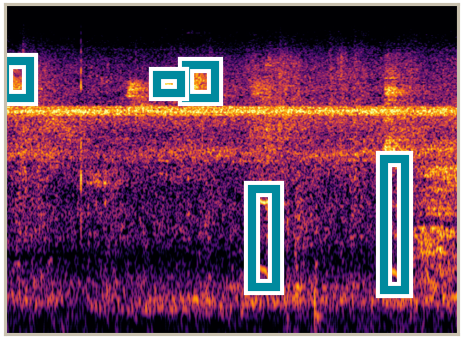
\includegraphics[height=34mm]{pipeline_detecciones}};
  \end{tikzpicture}
\end{frame}

% --------------------------------------------------------------------------------------------
\begin{frame}{How the model works}
  \centering
  \begin{tikzpicture}[
      stage/.style={inner sep=0pt},
      label/.style={font=\scriptsize, color=muted, align=center, anchor=north},
      flow/.style={-{Stealth[length=2.2mm]}, line width=0.9pt, color=match},
    ]
    \node[stage] (audio) {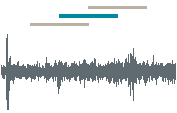
\includegraphics[height=23mm]{pipeline_audio}};
    \node[stage, right=6mm of audio] (mel) {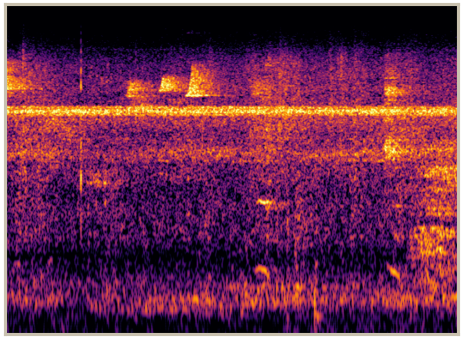
\includegraphics[height=23mm]{pipeline_espectrograma}};
    \node[right=6mm of mel, fill=ink, rounded corners=2mm, minimum height=23mm,
          minimum width=19mm, text=white, align=center, font=\small\bfseries] (yolo)
          {YOLO26s\\[1mm]{\tiny\mdseries\color{tierlow}detector}};
    \node[stage, right=6mm of yolo] (det) {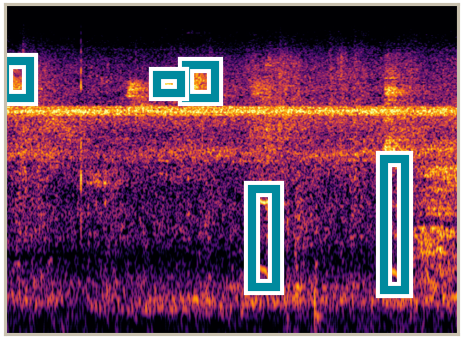
\includegraphics[height=23mm]{pipeline_detecciones}};
    \draw[flow] (audio) -- (mel);
    \draw[flow] (mel) -- (yolo);
    \draw[flow] (yolo) -- (det);
    \node[label] at (audio.south) {Recording, cut into\\3\,s windows (1.5\,s hop)};
    \node[label] at (mel.south) {Log-mel spectrogram};
    \node[label] at (yolo.south) {\vphantom{L}};
    \node[label] at (det.south) {Box, species,\\call type, score};

    % La tabla de Raven que sale de esa ventana
    \node[anchor=north east, inner sep=0pt] (raven) at ($(det.south east)+(0,-13mm)$) {%
      \tiny\color{ink}%
      \begin{tabular}{@{}rrrrllr@{}}
        \toprule
        \textbf{Begin} & \textbf{End} & \textbf{Low Hz} & \textbf{High Hz} & \textbf{Sp.} &
        \textbf{Call} & \textbf{Score} \\
        \midrule
        % generado por notebook/figuras_presentacion.ipynb; no editar
21.00 & 21.17 & 7,825 & 11,829 & SB & PPC & 0.25 \\
22.01 & 22.17 & 8,251 & 10,161 & SB & PPC & 0.58 \\
22.20 & 22.40 & 7,860 & 11,333 & SB & PPC & 0.65 \\
22.64 & 22.80 & 485 & 2,594 & SM & CC & 0.43 \\
23.51 & 23.65 & 441 & 3,793 & SM & CC & 0.21
\\
        \bottomrule
      \end{tabular}};
    \node[anchor=south east, font=\scriptsize, color=muted, inner sep=0pt]
      at ($(raven.north east)+(0,1.2mm)$) {Raven selection table};

    % Las cifras globales, a la izquierda de la tabla
    \node[anchor=north west, inner sep=0pt] at ($(audio.south west)+(0,-13mm)$) {%
      \metric{\recall}{recall}%
      \metric{\precision}{precision}%
      \metric{\mapThirty}{mAP@0.3}%
      \metric{\speciesCorrect\,\%}{right species}};
  \end{tikzpicture}

  \vfill
  \raggedright{\tiny\color{muted}Test set: \testBoxes{} annotated calls in \testRecordings{}
  recordings \textperiodcentered{} detections with score $\geq$ \threshold{} \textperiodcentered{}
  a hit overlaps an annotation with IoU $\geq$ 0.3 \textperiodcentered{} chosen among
  \nModels{} architectures \textperiodcentered{} \realtime$\times$ faster than real time on
  one GPU}
\end{frame}

% --------------------------------------------------------------------------------------------
\begin{frame}{Performance by species}
  \vspace*{-1mm}
  {\small\color{muted}\nCovered{} of \nTrained{} trained call types reach 0.80 recall
  (\coveredShare\,\% of test calls) \textperiodcentered{} \nNotTrained{} were left out}
  \par\vspace{2.5mm}
  % generado por notebook/figuras_presentacion.ipynb; no editar
\speciescard{PT}{P.~toppini}{0.95}{705}{%
  \callrow{sqc}{0.993}{0.672}{tierhigh}{\textbf{0.99}}
  \callrow{dc*}{0.942}{0.905}{tierhigh}{\textbf{0.94}}}%
  {\nottrained{\code{ac}~44 \textperiodcentered{} \code{pp}~43 \textperiodcentered{} \code{bp}~39}}%
\hfill
\speciescard{AS}{A.~sara}{0.87}{2,668}{%
  \callrow{hc*}{0.947}{0.831}{tierhigh}{\textbf{0.95}}
  \callrow{bc}{0.617}{0.669}{tiermid}{0.62}}%
  {}%
\hfill
\speciescard{AA}{A.~azarae}{0.80}{366}{%
  \callrow{gc}{0.807}{0.485}{tierhigh}{\textbf{0.81}}
  \callrow{hm}{0.795}{0.761}{tierhigh}{\textbf{0.80}}
  \callrow{sc}{0.755}{0.690}{tiermid}{0.75}}%
  {}%
\hfill
\speciescard{LW}{L.~weddelli}{0.79}{1,178}{%
  \callrow{sqc}{0.865}{0.634}{tierhigh}{\textbf{0.87}}
  \callrow{ta}{0.857}{0.639}{tierhigh}{\textbf{0.86}}
  \callrow{cs}{0.813}{0.710}{tierhigh}{\textbf{0.81}}
  \callrow{vc}{0.800}{0.451}{tierhigh}{\textbf{0.80}}
  \callrow{trino}{0.648}{0.486}{tiermid}{0.65}}%
  {\nottrained{\code{cc}~phrase \textperiodcentered{} \code{aa}~80 \textperiodcentered{} \code{phc}~34}}%
\par\vspace{2mm}
\speciescard{AC}{A.~chamek}{0.76}{1,020}{%
  \callrow{bc}{0.820}{0.750}{tierhigh}{\textbf{0.82}}
  \callrow{chc}{0.720}{0.567}{tiermid}{0.72}
  \callrow{sc}{0.389}{0.677}{tierlow}{0.39}
  \callrow{gc}{0.339}{0.594}{tierlow}{0.34}}%
  {\nottrained{\code{whc}~35 \textperiodcentered{} \code{cc}~29}}%
\hfill
\speciescard{SM}{S.~macrocephalus}{0.73}{1,143}{%
  \callrow{cc}{0.847}{0.595}{tierhigh}{\textbf{0.85}}
  \callrow{fs}{0.625}{0.525}{tiermid}{0.62}
  \callrow{hic}{0.593}{0.548}{tierlow}{0.59}
  \callrow{pc}{0.518}{0.413}{tierlow}{0.52}
  \callrow{sc}{0.304}{0.459}{tierlow}{0.30}}%
  {\nottrained{\code{fc}~phrase \textperiodcentered{} \code{whc}~76 \textperiodcentered{} \code{acc}~8}}%
\hfill
\speciescard{SB}{S.~boliviensis}{0.72}{851}{%
  \callrow{spc}{0.776}{0.455}{tiermid}{0.78}
  \callrow{pcc}{0.710}{0.507}{tiermid}{0.71}
  \callrow{ppc}{0.692}{0.411}{tiermid}{0.69}
  \callrow{sc}{0.676}{0.368}{tiermid}{0.68}}%
  {\nottrained{\code{pcs}~phrase}}%
\hfill
\emptycard{CC}{C.~cuscinus}{29}{7}%
\par
  \vfill
  {\tiny\color{muted}Bar: recall on the test set \textperiodcentered{} \diamondmark{} precision
  \textperiodcentered{} \hatch{} not trained: annotation count (under \minCount) or a phrase
  label \textperiodcentered{} * whole-window call}
  \begin{tikzpicture}[remember picture, overlay]
    \node[anchor=north east, inner sep=0pt, font=\scriptsize, color=muted]
      at ($(current page.north east)+(-8mm,-7.6mm)$)
      {\swatch{tierhigh}\,{\color{ink}\bfseries$\geq$\,0.80 covered}\quad
       \swatch{tiermid}\,0.60--0.80 partial\quad
       \swatch{tierlow}\,$<$\,0.60 weak};
  \end{tikzpicture}
\end{frame}

% --------------------------------------------------------------------------------------------
\begin{frame}{Detections vs.\ delivered annotations}
  \vspace*{-1mm}
  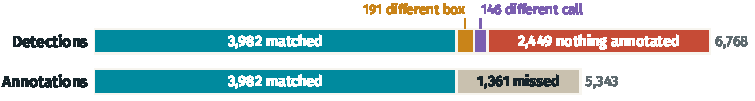
\includegraphics[width=\linewidth]{contraste}
  \par\vspace{2mm}
  \showcase{boxdiff}{Different box}{\nBox}{ejemplo_box}%
    {Same \code{sm/fs} syllables: the team boxed them tight, the model tall.}\hfill
  \showcase{nothing}{Nothing annotated}{\nNone}{ejemplo_none}%
    {Two alike \code{lw/ta} alarms; only the right one was annotated. Missed call or noise?}\hfill
  \showcase{calldiff}{Different call}{\nLabel}{ejemplo_label}%
    {Annotated \code{lw/trino}, detected \code{lw/vc}. \labelSameSpecies\,\% stay in the
    species.}
  \par\vfill
  {\tiny\color{muted}Test set, whole-window calls excluded \textperiodcentered{} dashed: team
  annotation \textperiodcentered{} solid: model detection}
\end{frame}

% --------------------------------------------------------------------------------------------
\begin{frame}{Continuous improvement loop}
  \centering
  \begin{tikzpicture}[
      stage/.style={draw=rule, fill=white, rounded corners=3mm, line width=0.5pt,
                    minimum width=48mm, minimum height=15mm, align=left,
                    inner xsep=9mm, inner ysep=2mm, font=\small},
      flow/.style={-{Stealth[length=2.6mm]}, line width=1.2pt, color=match},
    ]
    \node[stage] (detect) at (-37mm, 17mm)
      {\textbf{Model detects}\\[0.5mm]{\scriptsize\color{muted}new recordings $\to$ Raven tables}};
    \node[stage] (review) at (37mm, 17mm)
      {\textbf{Team validates}\\[1mm]%
       \chip{match}{TP}\,\chip{nothing}{FP}\,\chip[ink]{missed}{FN}\,\chip{ink}{TN}\,%
       \chip{boxdiff}{box}\,\chip{calldiff}{call}};
    \node[stage] (clean) at (37mm, -17mm)
      {\textbf{Clean data}\\[0.5mm]{\scriptsize\color{muted}more, consistent annotations}};
    \node[stage] (retrain) at (-37mm, -17mm)
      {\textbf{Retrain}\\[0.5mm]{\scriptsize\color{muted}same pipeline, same test set}};
    \node[badge=match] at (detect.west) {\faIcon{wave-square}};
    \node[badge=ink] at (review.west) {\faIcon{user-check}};
    \node[badge=tierhigh] at (clean.west) {\faIcon{database}};
    \node[badge=calldiff] at (retrain.west) {\faIcon{cogs}};

    \draw[flow] (detect.east) -- ($(review.west)+(-5.5mm,0)$);
    \draw[flow] (review.south) -- (clean.north);
    \draw[flow] ($(clean.west)+(-5.5mm,0)$) -- (retrain.east);
    \draw[flow] (retrain.north) -- (detect.south);

    \node[align=center] at (0,0) {{\Huge\color{match}\faIcon{sync-alt}}\\[2mm]
      {\small\bfseries better data}\\{\small\bfseries better model}};
  \end{tikzpicture}

  \vfill
  \raggedright{\scriptsize\color{muted}\textbf{First round:} review the \corpusNone{} detections
  with nothing annotated (half are in \corpusNoneHalf{} recordings) \textperiodcentered{} one box
  rule for \code{sm/fs} \textperiodcentered{} \ccMissing{} more \code{cc/cc} calls to reach
  \minCount}
\end{frame}

% --------------------------------------------------------------------------------------------
\begin{frame}[plain]
  \vspace*{12mm}
  {\fontsize{30}{34}\selectfont\bfseries Thank you}\par\vspace{4mm}
  {\large\color{muted}Questions and feedback are welcome}\par\vspace{12mm}
  {\small\color{muted}\insertauthor\quad\textperiodcentered\quad\texttt{\repoUrl}}
  \begin{tikzpicture}[remember picture, overlay]
    \node[anchor=east, inner sep=0pt, text=match!25] at ($(current page.east)+(-16mm,0)$)
      {\fontsize{90}{90}\selectfont\faIcon{sync-alt}};
  \end{tikzpicture}
\end{frame}

\appendix

% --------------------------------------------------------------------------------------------
\begin{frame}{Appendix \textperiodcentered{} Four architectures trained}
  \vspace*{-1mm}
  {\small\color{muted}Same data, same splits, same protocol; each at its own validation
  threshold, measured on the test set}
  \par\vspace{3mm}
  {\scriptsize\setlength{\tabcolsep}{3pt}\renewcommand{\arraystretch}{1.25}%
  \begin{tabular}{@{}l l r c r r r r@{}}
    \toprule
    \textbf{Architecture} & \textbf{Pretrained} & \textbf{Params} &
    \textbf{Recall, 95\,\% CI} & \textbf{Recall} & \textbf{Precision} & \textbf{mAP@0.3} &
    \textbf{GPU min} \\
    & & {\tiny\color{muted}millions} & \ciaxis & & & & {\tiny\color{muted}per hour of audio} \\
    \midrule
    \rawinput{figures/tablas/modelos.tex} \\
    \bottomrule
  \end{tabular}}
  \par\vfill
  {\scriptsize\color{muted}The recall intervals overlap: no architecture is measurably
  better at finding calls. YOLO26s leads on mAP@0.3 and is the cheapest to run, so it is the
  one in use.}
  \par\vspace{1mm}
  {\tiny\color{muted}Sorted by mAP@0.3 \textperiodcentered{} CI: bootstrap over recordings
  \textperiodcentered{} GPU time on one \gpuName}
\end{frame}

% --------------------------------------------------------------------------------------------
\begin{frame}{Appendix \textperiodcentered{} More detections with nothing annotated}
  \vspace*{-1mm}
  {\small\color{muted}The highest-scoring one per species, test set. Missed call or noise?}
  \par\vspace{3mm}
  % generado por notebook/figuras_presentacion.ipynb; no editar
\moreexample{sin_anotacion_1}{ac/chc}{0.85}{20240227\_090548}{45.5}%
\hfill
\moreexample{sin_anotacion_2}{lw/trino}{0.85}{20240125\_162433}{2.4}%
\hfill
\moreexample{sin_anotacion_3}{sm/fs}{0.86}{20240615\_120621}{25.2}%
\par\vspace{2.5mm}
\moreexample{sin_anotacion_4}{sb/sc}{0.81}{20240202\_165826}{2.5}%
\hfill
\moreexample{sin_anotacion_5}{as/bc}{0.79}{20240621\_074544}{19.2}%
\hfill
\moreexample{sin_anotacion_6}{aa/sc}{0.76}{20240117\_051239}{184.9}%

  \par\vfill
  {\tiny\color{muted}Solid: the model detection \textperiodcentered{} dashed: team annotations
  nearby \textperiodcentered{} recording @ second where the box starts}
\end{frame}

\end{document}
